\chapter{Application for design-space~exploration}
\label{chap:apply}

To achieve our goal of supporting design-space exploration with stochastic metrics, a formalism for the convenient modular construction of stochastic models was presented in the previous chapters along with a technique for transforming engineering (architectural) models into stochastic models. Now the application of these tools in design-space exploration (\textabbr{DSE}) toolchains is discussed.

\citet{Kang10effective} have identified cornerstones of an effective \textabbr{DSE} framework as
\begin{inparaenum}
\item a suitable \emph{representation} of the design space,
\item \emph{analysis} capabilities to check discovered potential candidates against design constraints and
\item an \emph{exploration method} for navigating interesting solutions.
\end{inparaenum}
The approaches and representations used for \textabbr{DSE} in the context of model-driven engineering were further classified by \citet{Vanherpen14patterns}. They have identified the following \emph{\textabbr{DSE} patterns} of exploration methods:
\begin{itemize}
\item The \emph{Model Generation Pattern} synthesizes design candidates that satisfy a set of constraints, which are imposed imposed based on the metamodel and in addition by the designer. During the exploration, design candidates are represented as solutions of a constraint satisfaction problem.
\item The \emph{Model Adaptation Pattern} constructs an exploration representation, such as a string of genes in genetic algorithms~\todo*{cite}, from an initial model provided by the designer. Based on the guidance of a goal function further design candidates are devised in this intermediate form using (meta-)heuristic search.
\item The \emph{Model Transformation Pattern} directly represents the design candidates as an instance model. Model transformation rules that yield alternative models are scheduled using (meta-)heuristics to optimize a goal function.
\item The \emph{Exploration Chaining Pattern} adds multiple abstraction layers to \textabbr{DSE} to prune the space of alternative solutions. At each abstraction layer, an exploration pattern is used to prune non-feasible solutions while selecting feasible solutions to be refined in the next layer. Domain knowledge is used to define abstraction layers. Costly evaluation of design candidates is usually deferred to the lower layers.
\end{itemize}
\citet{Vanherpen14patterns} also classified the representations employed by \textabbr{DSE} patterns:
\begin{enumerate}
\item The starting point for exploration is expressed in a \emph{model} formalism.
\item Constraints to be satisfied by the design alternatives and objective function to be optimized are captured by \emph{constraint} and \emph{goal} formalisms.
\item Design candidates are stored in an \emph{exploration formalism} during the exploration. In the \emph{Model Transformation Pattern}, this coincides with the \emph{model} formalism.
\item The exploration formalism may be transformed into an \emph{analysis} formalism to check feasability with respect to the constraints.
\item A second transformation may target a \emph{performance} formalism to check optimality with respect to the goal functions.
\item Execution traces yielding the design alternatives are stored in a \emph{trace} formalism.
\item Finally, the solution is output in a \emph{solution} formalism, which may coincide with either the model or the trace formalism.
\end{enumerate}

The \textabbr{RGSPN} formalism proposed in \cref{chap:rgspn} may serve as both an \emph{analysis} formalism when constraints are formulated in terms of stochastic analysis queries and as a \emph{performance} formalism when the optimized goal function is a stochastic metric. Hence in \textabbr{DSE} the transformation proposed in \cref{chap:transform} should be employed as a means of transformin models in the \emph{exploration} formalism to the \emph{analysis} formalism. In more elaborate transformation chains, where a separate analysis formalism is employed and \textAbbr{RGSPN}s are only used as \emph{performance} formalism, the \emph{analysis} formalism may serve as a source instead. The traceability links produced by the transformation ensure that the results of the analysis can be intepreted as information about the satisfaction of constraints and the values of goal functions defined over the engineering formalisms.

\citep{Varro17generation}

\todo*{}

\section{Integration with design-space exploration toolchains}

\begin{figure}
  \centering
  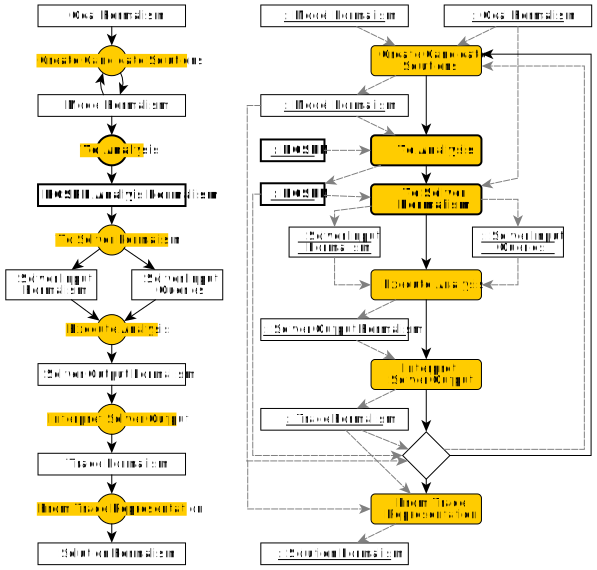
\includegraphics[scale=0.9]{figures/dse_ftg_pm}
  \caption{Formalism transformation graph and process model of the \emph{Model Transformation} \textabbr{DSE} pattern with \textabbr{RGSPN}-based analysis. The components in \emph{bold} were implemented in our work, while the rest of the components should be supplied by the \textabbr{DSE} framework and stochastic analysis tool.}
\end{figure}

\subsection{Design-space explorers}

\subsection{Formal analysis tools}

\section{Software implementation}

A software tool for the development of transformation specifications and their execution was implemented as a plug-in for the Eclipse Oxygen.1 Integrated Development Environment~(\textabbr{IDE}). The plug-in is based on open source technologies from the Eclipse Modeling Project: the \emph{Eclipse Modeling Foundation}~(\textabbr{EMF}), the \emph{XText} framework for language engineering and \emph{\textabbr{VIATRA}} scalable reactive model queries and transformations.\todo{Cite the relevant technologies, or use \textabbr{URL} footnotes?}

The software consists of two major components. Both \textabbr{RGSPN} modules and model transformations from arbitrary \textabbr{EMF}-based \textAbbr{DSL}s to \textAbbr{RGSPN}s can be developed in the transformation specification environment. The transformation can be executed either inside the \textabbr{IDE} for testing or inside a \textabbr{DSE} program after Java code generation. Together with a runtime library implementing the transformation engine, the generated Java code provides incremental transformation from the engineering \textAbbr{DSL} to stochastic Petri nets.

\subsection{Specification environment}

\subsection{Transformation execution}

\section{Evaluation of incremental transformations}

We carried out preliminary scalability evaluation of our transformation runtime in order to study the overhead the imposed on transformation imposes on design-space exploration. Both \emph{batch execution}---where the transformation engine is initially instantiated and the intermediate and target \textabbr{RGSPN} models are materialized according to the engineering models---and \emph{incremental execution}---where each source model change is immediately translated into intermediate and target model changes---were studied. More specifically, we carried out the evaluation in the \emph{dining philosophers} domain to address three research questions:
\begin{description}
\item[\textabbr{RQ1}] How does the initial batch transformation from the engineering \textabbr{DSL} to the formal stochastic model (\textabbr{GSPN}) scale with respect to size of the input model?
\item[\textabbr{RQ2}] How does the incremental transformation scale with respect to the size and the change operations of the input model?
\item[\textabbr{RQ3}] What is the overhead associated with the serialization of models to the \textabbr{ISO}/\textabbr{IEC} \textabbr{PNML} interchange format?
\end{description}

Answering these questions may help identifying strengths and weaknesses of the proposed approach to the stochastic evaluation of engineering models. Moreover, the answers to \textbf{\textabbr{RQ1}} and  \textbf{\textabbr{RQ2}} aid in determining whether incremental or batch model transformation should be used according to the usual size of source changes. This choice arises when there is no need to construct the target model change as a sequence of operations for each source change; therefore incremental execution is not necessitated and the system integrator can chose between either execution schemes. Lastly, the answer to \textbf{\textabbr{RQ3}} tells whether the overhead of serialization into a portable format is acceptable or more direct integration and communication with the external solver is needed.

\subsection{Measurement setup}

\begin{table}
  \caption{Source model, abstract net and concrete net sizees for the philosophers models.}
  \label{tbl:apply:model-size}
  \sisetup{table-number-alignment=center}
  \centering
  \begin{tabular}{@{}rS[table-format=3.0]S[table-format=5.0]S[table-format=4.0]@{}}
    \toprule
    \(N\) & \multicolumn{1}{c}{\#Source} & \multicolumn{1}{c}{\#Abstract net} & \multicolumn{1}{c@{} }{\#Concrete net} \\
    \midrule
    \(8\) & 9 & 644 & 532 \\
    \(16\) & 17 & 1268 & 1060 \\
    \(32\) & 33 & 2516 & 2116 \\
    \(64\) & 65 & 5012 & 4228 \\
    \(128\) & 129 & 10004 & 8452 \\
    \bottomrule
  \end{tabular}
\end{table}

Measurements were performed on instances of the \emph{dining philosophers} domain model, which was used throughout this work as a running example. The number of philosophers and thus the size of the source model was set to \(N = 8\), \(16\), \(32\), \(64\) and \(128\). \Cref{tbl:apply:model-size} shows the sizes of the source models, as well as the sizes of the derived intermediate abstract \textAbbr{RGSPN}s and target concrete \textAbbr{RGSPN}s, including any symbol, edge and expression objects.

To evaluate incremental execution, various \emph{change operations} were defined as follows:
\begin{itemize}
\item \textbf{Swap} rotates the seating order two philosophers adjacent around the table. This change only modifies references in the source model; hence is simulates a \textabbr{DSE} rule with no object creation and deletion.
\item \textbf{New} creates a new philosopher and inserts it between two existing philosophers.
\item \textbf{Delete} removes a philosopher from the table and deletes it from the model.
\item \textbf{Fixed\-Mix} simulates a compound model change of fixed size by a randomly ordered mixture of \(8\)~\textbf{swap}, \(4\)~\textbf{new} and \(4\)~\textbf{delete} operations.
\item \textbf{Scaled\-Mix} simulates a compound model change of model-dependent size by a randomly ordered mixture of \(N\)~\textbf{swap}, \(\frac{N}{2}\)~\textbf{new} and \(\frac{N}{2}\)~\textbf{delete} operations.
\end{itemize}

The compound model change \textbf{scaled\-Mix} was devised such that half of the philosophers is replaced around the table, while \textbf{fixed\-Mix} is obtained from \textbf{scaled\-Mix} by setting \(N = 8\) to the size of the smallest input model. The model elements involved in the simple and compound model changes were randomized similarly to the order of simple operations without compound ones. However, the random seed was fixed for each measurements, i.e.~the model changes are always deterministic given the input model size.

Measurements of a given execution scheme and change type comprise a \emph{scenario}. Batch transformation of the initial models was studied in an additional scenario without any model change. Every scenario was executed for each model size \(N \in \{8, 16, 32, 64, 128\}\) multiple times. A single execution of the transformation is an \emph{iteration}. After 10 warm-up iterations, the run times of 30 iterations were measured for each scenario and model size.

To avoid measuring the latency of the hard disk, the target \textabbr{GSPN} models were serialized in the \textabbr{PNML} format to an in-memory output stream. However, for externals tools that can only read Petri nets from a disk, an in-memory file system may be needed instead.

Measurements were performed on a workstation with two Intel Xeon 5160 dual-core 3.00\thinspace GHz processors and 16\thinspace GB memory. The heap size of the Java 1.8u144 virtual machine was limited to 8\thinspace GB with a 30\thinspace s wall clock time limit for each iteration.

\subsection{Results}

\begin{figure}
  \centering
  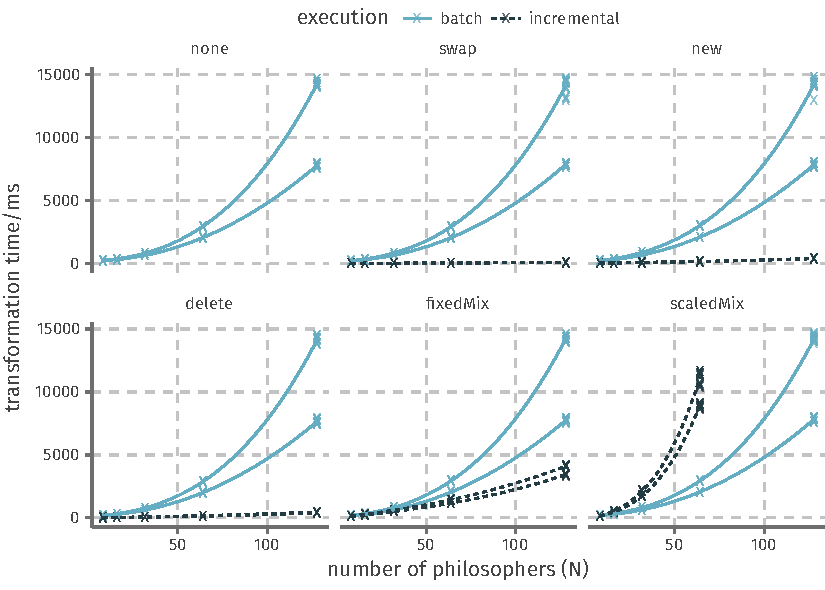
\includegraphics{figures/plot_execution}
  \caption{Execution times of transformations.}
  \label{fig:apply:plot-execution}
\end{figure}

The execution time of the transformations on the various model sizes and change operations is shown in the scatter plot in \cref{fig:apply:plot-execution}. It is apparent that the distribution of run times is extremely bimodal, especially for larger source models.

Therefore instead of fitting a single curve for each scenario, data points were split into two clusters for each scenario and model size. First the threshold \(\textit{thresh} = \frac{\textit{max} - \textit{min}}{2}\) was determined, where \textit{max} and \textit{min} were the smallest and largest execution times, respectively. Due to the heavy bimodality, no data points were adjacent to this threshold. The upper and lower clusters were then formed by data points above and below \textit{thresh}. The upper and lower curves of degree up \(3\), which are shown in \cref{fig:apply:plot-execution}, were fit to data points from the upper and lower clusters of each scenario. It is apparent that execution times of the batch scenarios in both the upper are lower clusters scale superlinearly, and the same phenomemon also occurs with incremental view synchronization of mixes of change operations. There was no correlation between the iteration numbers and the clusters, i.e.~the bimodality was not found to be a warm-up transient artifact.

\begin{table}
  \caption{Minimum and maximum execution times of transformations/ms.}
  \label{tbl:apply:minmax}
  \centering
  \begin{tabular}{@{}r*{6}{r@{\,}c@{\,}r}@{}}
    \toprule
    & & & & \multicolumn{15}{c@{}}{Incremental} \\
    \cmidrule{5-19}
    \(N\) & \multicolumn{3}{c}{Batch}  & \multicolumn{3}{c}{Swap}  & \multicolumn{3}{c}{New}  & \multicolumn{3}{c}{Delete}  & \multicolumn{3}{c}{FixedMix} & \multicolumn{3}{c@{}}{ScaledMix} \\
    \midrule
    \(8\)&\(209\)&--&\(294\)&\(6\)&\(\updownarrow\)&\(9\)&\(15\)&\(\updownarrow\)&\(26\)&\(17\)&--&\(33\)&\(126\)&\(\updownarrow\)&\(166\)&\(124\)&\(\updownarrow\)&\(163\)\\
    \(16\)&\(281\)&\(\updownarrow\)&\(344\)&\(8\)&\(\updownarrow\)&\(15\)&\(23\)&\(\updownarrow\)&\(41\)&\(27\)&\(\updownarrow\)&\(45\)&\(224\)&\(\updownarrow\)&\(291\)&\(456\)&\(\updownarrow\)&\(575\)\\
    \(32\)&\(631\)&\(\updownarrow\)&\(852\)&\(13\)&\(\updownarrow\)&\(18\)&\(46\)&\(\updownarrow\)&\(91\)&\(51\)&\(\updownarrow\)&\(86\)&\(505\)&\(\updownarrow\)&\(631\)&\(1714\)&\(\updownarrow\)&\(2221\)\\
    \(64\)&\(2006\)&\(\updownarrow\)&\(2975\)&\(26\)&\(\updownarrow\)&\(34\)&\(119\)&--&\(164\)&\(129\)&\(\updownarrow\)&\(181\)&\(1148\)&\(\updownarrow\)&\(1473\)&\(8644\)&\(\updownarrow\)&\(11\thinspace681\)\\
    \(128\)&\(7568\)&\(\updownarrow\)&\(14\thinspace659\)&\(52\)&\(\updownarrow\)&\(68\)&\(357\)&\(\updownarrow\)&\(427\)&\(383\)&\(\updownarrow\)&\(478\)&\(3342\)&\(\updownarrow\)&\(4211\) & \multicolumn{3}{c@{}}{Timed out}\\
    \bottomrule
  \end{tabular}
\end{table}

The minimum and maximum execution times of each scenario and model size, which are representative of the execution times in two clusters, are shown in \cref{tbl:apply:minmax}. Because the considered model changes did not affect the run times of batch transformations, we only report the run time of the batch transformation of the initial model. The symbol \(\updownarrow\) indicates significant (\(p < 0.05\)) bimodality of the execution time distributions according to Hartigan's dip test~\citep{Maechler16diptest}, while~--~denotes unimodal distributions.

In order to study the source of bimodality in the execution times, a further experiment was conducted. The batch transformations, which had the most striking bimodality, was executed with further instrumentation on the source model containing \(N = 128\) philosophers. Four stages of the transformation were distinguished:
\begin{enumerate}
\item The \emph{view query} phase prepares the model queries that are the preconditions of the view transformation. In \textabbr{VIATRA} Query, this corresponds to the construction of an appropriate \textabbr{RETE} net~\todo*{cite?} and the traversal of the source model to populate the base relations.
\item The \emph{view transformation} phase fires the transformation rules on the \textabbr{VIATRA} Event-driven Virtual Machine (\textabbr{EVM}) to construct the abstract \textabbr{RGSPN} model with references.
\item The \emph{concretizer query} phase traverses the abstract net to prepare the precondition queries of the concretizer transformation.
\item The \emph{concretizer transformation} phase is ran on the \textabbr{EVM} to resolve references and inline expression in the abstract net to construct the concrete \textabbr{RGSPN} target model.
\end{enumerate}
In ordinary transformation execution, the query phases are ran simultaneously to avoid spurious model traversal. Moreover, the transformation phases share an \textabbr{EVM} execution schema that provides sequential execution by prioritized firing of transformation rules. However, in our experiment, we separated the phases to observe their run times individually.

\begin{figure}
  \centering
  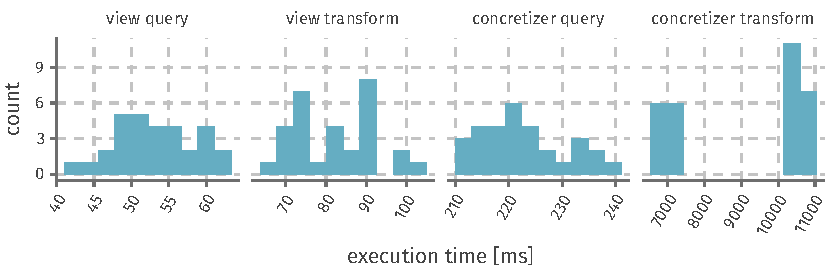
\includegraphics{figures/plot_histogram}
  \caption{Execution times of batch transformation phases with \(N = 128\) philosophers.}
  \label{fig:apply:histogram}
\end{figure}

The histogram of the transformation phases with 30~iterations is shown in \cref{fig:apply:histogram}. The concretizer transformation phase, which is running an order of magnitude slower than other phases, is revealed as the source of the heavy bimodality.

\begin{table}
  \caption{Execution times of \textabbr{PNML} serializations.}%
  \label{tbl:apply:serialization}%
  \begin{minipage}{0.5\textwidth}%
    \centering
    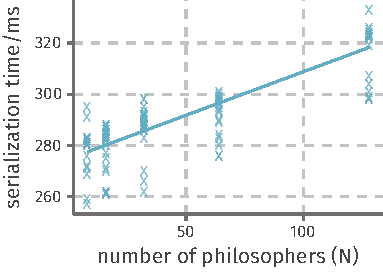
\includegraphics{figures/plot_serialization}%
  \end{minipage}%
  \begin{minipage}{0.5\textwidth}%
    \centering
    \begin{tabular}{@{}rr@{\,}c@{\,}lS[table-number-alignment=center,table-format=6.0]@{}}
      \toprule
      \(N\) & \multicolumn{3}{c}{Time/ms} & \multicolumn{1}{c@{}}{\textabbr{PNML} size/bytes} \\
      \midrule
      \(8\) & \(257\) & -- & \(295\) & 50700 \\
      \(16\) & \(261\) & \(\updownarrow\) & \(288\) & 100441 \\
      \(32\) & \(262\) & -- & \(298\) & 200572 \\
      \(64\) & \(276\) & -- & \(301\) & 400736 \\
      \(128\) & \(298\) & -- & \(333\) & 802454 \\
      \bottomrule
    \end{tabular}%
  \end{minipage}%
\end{table}

Lastly, the time taken by serialization of the target models in \textabbr{ISO}/\textabbr{IEC} \textabbr{PNML} format to an in-memory output stream is show in \cref{tbl:apply:serialization} and the accompanying figure. Both the serialization time and the size of the resulting \textabbr{PNML} descriptions scale linearly with the model size. Significant bimodality was detected by the dip test on in the case of \(N = 16\) with \(p = 0.004\). However, it is possible the latter observation is only due to pure randomness.

\subsection{Observations}

The research questions \textbf{\textabbr{RQ1}--3} may be answered based on the presented measurement results as follows:
\begin{description}
\item[\textabbr{RQ1}] Batch transformations scaled superlinearly in the size of the input model. Transformation of the largest studied source model, which had 129 elements, took up to 15\thinspace s to produce a 8452-element output model along with traceability information which affords incremental synchronization of the target \textabbr{RGSPN} according to future source model changes.

  The run time exhibited significats bimodality, apparent to both visual examination an Hartigan's dip test of bimodality. In the most extreme case of \(N = 128\) philosophers, iterations in the upper cluster of run times took nearly twice as long a those in the lower cluster, while for smaller input models, the difference was up to 50\%.
\item[\textabbr{RQ2}] Incremental synchronization of the \textbf{swap} change operation was found to take linear time as the function of the source model time. Therefore the synchronization time depends on not only the changes to be synchronized but also on the size of the input model. Synchronization time for \textbf{create} and \textbf{delete} changes was found to be superlinear similarly to the batch transformation. This indicates the the creation and removal of objects has larger overhead than the modification of references in the source model and the transformed \textabbr{RGSPN}.

  Synchronization time was below that of batch transformation in the \textbf{fixed\-Mix} compound change operation. However, for the change operation \textbf{scaled\-Mix} of model-dependent size, batch transformation was found to be faster that incremental synchronization in all cases except \(N = 8\). Therefore we can conclude that if change operations affect large portions of the input model batch transformation may be more economical than incremental synchronization; although for smaller input changes, synchronization won by a margin of at least 14\%, the smallest difference being achieved on the \textbf{fixed\-Mix} change with \(N = 16\).
\item[\textabbr{RQ3}] The \textabbr{PNML} serialization routine, which traverses the concrete \textabbr{RGSPN} model to produce its \textabbr{PNML} equivalent, scaled linearly in the size of the input model. However, the cause of this phenomemon is probably that the size of concrete \textabbr{GSPN} itself is only a constant multiple of the input model size. The size of the generated \textabbr{PNML} was also a multiple of the input model size. In all measured cases \textabbr{PNML} serialization took no more than \(\nicefrac{1}{3}\) of a second, much less than the time taken by analysis tools to analyze stochastic Petri net models similar to the ones considered. Therefore \textabbr{PNML} serialization is not a significant overhead compared to stochastic analysis. It is also generally smaller than the time taken by batch transformation.
\end{description}

Bimodality of transformation run time distributions was found to be caused by the execution of the \textabbr{RGSPN} concretizer transformation on the \textabbr{VIATRA} Event-driven Virtual Machine. We hyphotesize that the large differences is execution time are caused by the nondeterministic scheduling in \textabbr{EVM}.

While conflicting transformation rules of differing priorities are fired in the order of their priorities, the ordering between rules of the same priority are not defined. The firing of a low-priority rule may activate a higher priority one. In the implementation of our concretizer transformation, the work performed by some high-priority rules may be occasionally undone by a low-priority rule when \textabbr{RGSPN} references are resolved and expressions are inlined due to the dependency tracking required for for expression inlining. Thus if low-priority rules are fired in an unsuitable order, some work must be redone by high-priority rules after the corrent dependencies are taken into account. Although taking dependencies between \textabbr{RGSPN} symbols and expressions at the level of \textabbr{EVM} conflict resolution may alleviate this issue, performing such tracking efficiently remains in the scope of future work.

Due to the hashing employed by the conflict resolver, the firing order of equal priority rules is determined at runtime by \texttt{hashCode()} of the rule activation objects, which is not overridden from its default implementation. In the Java runtime environment, the default \texttt{hashCode()} is connected with the allocation of objects and forcing it to be deterministic for the sake of consistent measurements is difficult. Hence the apparently random switching between fast and slow execution of the concretizer transformation.

\subsection{Threats to validity}

An internal threat to validity was the possibility of an incorrect implementation of the transformation engine or the incorrect description of the transformation from the dining philosophers domain model to Petri nets. To ensure correctness the transformation outputs were manually inspected for the small source models for consistency with the source models and the transformation description.

Moreover, interferences may have occurred in the measurement environment. To reduce interferences, the measurements were ran on a physical machine on which no other task was executed at the time. Each scenario and input model was measured 30 times after 10 warm-up iterations to reduce random noise and the interferences caused by ongoing just-in-time compilation. Garbage collection within the runtime enviroment was also controlled manually to ensure that subsequent iterations did not interfere.

Despite these attemps, run time distributions were found to be bimodal having two clusters with small variance instead of a single cluster with small variance. We conducted further measurements to break down the transformation into phases and hypothesize that this phenomenon is intrinsic to the current implementation of the transformation insteand of being caused by interferences.

As we conducted our expriments on in single domain with a single transformation description, several external threats to validity impede generalization. Firstly, further studies are needed to observe the behavior of the transformation on different domain models and transformation descriptions. Secondly, as the size of the target \textabbr{RGSPN} models was a constant multiple of the size of the source models, behaviors depending on the sizes of either of these models could not be distinguished from each other.
